%% abtex2-modelo-trabalho-academico.tex, v-1.9.5 laurocesar
%% Copyright 2012-2015 by abnTeX2 group at http://www.abntex.net.br/
%%
%% This work may be distributed and/or modified under the
%% conditions of the LaTeX Project Public License, either version 1.3
%% of this license or (at your option) any later version.
%% The latest version of this license is in
%%   http://www.latex-project.org/lppl.txt
%% and version 1.3 or later is part of all distributions of LaTeX
%% version 2005/12/01 or later.
%%
%% This work has the LPPL maintenance status `maintained'.
%%
%% The Current Maintainer of this work is the abnTeX2 team, led
%% by Lauro César Araujo. Further information are available on
%% http://www.abntex.net.br/
%%
%% This work consists of the files abntex2-modelo-trabalho-academico.tex,
%% abntex2-modelo-include-comandos and abntex2-modelo-references.bib
%%

% ------------------------------------------------------------------------
% ------------------------------------------------------------------------
% abnTeX2: Modelo de Trabalho Academico (tese de doutorado, dissertacao de
% mestrado e trabalhos monograficos em geral) em conformidade com
% ABNT NBR 14724:2011: Informacao e documentacao - Trabalhos academicos -
% Apresentacao
% ------------------------------------------------------------------------
% ------------------------------------------------------------------------

\documentclass[
	% -- opções da classe memoir --
	12pt,				% tamanho da fonte
	openright,			% capítulos começam em pág ímpar (insere página vazia caso preciso)
	twoside,			% para impressão em verso e anverso. Oposto a oneside
	a4paper,			% tamanho do papel.
	% -- opções da classe abntex2 --
	%chapter=TITLE,		% títulos de capítulos convertidos em letras maiúsculas
	%section=TITLE,		% títulos de seções convertidos em letras maiúsculas
	%subsection=TITLE,	% títulos de subseções convertidos em letras maiúsculas
	%subsubsection=TITLE,% títulos de subsubseções convertidos em letras maiúsculas
	% -- opções do pacote babel --
	english,			% idioma adicional para hifenização
	french,				% idioma adicional para hifenização
	spanish,			% idioma adicional para hifenização
	brazil				% o último idioma é o principal do documento
	]{abntex2}

% ---
% Pacotes básicos
% ---
\usepackage{lmodern}			% Usa a fonte Latin Modern
\usepackage[T1]{fontenc}		% Selecao de codigos de fonte.
\usepackage[utf8]{inputenc}		% Codificacao do documento (conversão automática dos acentos)
\usepackage{lastpage}			% Usado pela Ficha catalográfica
\usepackage{indentfirst}		% Indenta o primeiro parágrafo de cada seção.
\usepackage{color}				% Controle das cores
\usepackage{graphicx}			% Inclusão de gráficos
\usepackage{microtype} 			% para melhorias de justificação
% ---

% ---
% Pacotes adicionais, usados apenas no âmbito do Modelo Canônico do abnteX2
% ---
\usepackage{lipsum}				% para geração de dummy text
% ---

% ---
% Pacotes de citações
% ---
\usepackage[brazilian,hyperpageref]{backref}	 % Paginas com as citações na bibl
\usepackage[alf]{abntex2cite}	% Citações padrão ABNT

% ---
% CONFIGURAÇÕES DE PACOTES
% ---

% ---
% Configurações do pacote backref
% Usado sem a opção hyperpageref de backref
\renewcommand{\backrefpagesname}{Citado na(s) página(s):~}
% Texto padrão antes do número das páginas
\renewcommand{\backref}{}
% Define os textos da citação
\renewcommand*{\backrefalt}[4]{
	\ifcase #1 %
		Nenhuma citação no texto.%
	\or
		Citado na página #2.%
	\else
		Citado #1 vezes nas páginas #2.%
	\fi}%
% ---

% ---
% Informações de dados para CAPA e FOLHA DE ROSTO
% ---
\titulo{Modelo Canônico de\\ Trabalho Acadêmico com \abnTeX}
\autor{Equipe \abnTeX}
\local{Brasil}
\data{2015, v-1.9.5}
\orientador{Lauro César Araujo}
\coorientador{Equipe \abnTeX}
\instituicao{%
  Universidade do Brasil -- UBr
  \par
  Faculdade de Arquitetura da Informação
  \par
  Programa de Pós-Graduação}
\tipotrabalho{Tese (Doutorado)}
% O preambulo deve conter o tipo do trabalho, o objetivo,
% o nome da instituição e a área de concentração
\preambulo{Modelo canônico de trabalho monográfico acadêmico em conformidade com
as normas ABNT apresentado à comunidade de usuários \LaTeX.}
% ---


% ---
% Configurações de aparência do PDF final

% alterando o aspecto da cor azul
\definecolor{blue}{RGB}{41,5,195}

% informações do PDF
\makeatletter
\hypersetup{
     	%pagebackref=true,
		pdftitle={\@title},
		pdfauthor={\@author},
    	pdfsubject={\imprimirpreambulo},
	    pdfcreator={LaTeX with abnTeX2},
		pdfkeywords={abnt}{latex}{abntex}{abntex2}{trabalho acadêmico},
		colorlinks=true,       		% false: boxed links; true: colored links
    	linkcolor=blue,          	% color of internal links
    	citecolor=blue,        		% color of links to bibliography
    	filecolor=magenta,      		% color of file links
		urlcolor=blue,
		bookmarksdepth=4
}
\makeatother
% ---

% ---
% Espaçamentos entre linhas e parágrafos
% ---

% O tamanho do parágrafo é dado por:
\setlength{\parindent}{1.3cm}

% Controle do espaçamento entre um parágrafo e outro:
\setlength{\parskip}{0.2cm}  % tente também \onelineskip

% ---
% compila o indice
% ---
\makeindex
% ---

% ----
% Início do documento
% ----
\begin{document}

% Seleciona o idioma do documento (conforme pacotes do babel)
%\selectlanguage{english}
\selectlanguage{brazil}

% Retira espaço extra obsoleto entre as frases.
\frenchspacing

% ----------------------------------------------------------
% ELEMENTOS PRÉ-TEXTUAIS
% ----------------------------------------------------------
% \pretextual

% ---
% Capa
% ---
\imprimircapa
% ---

% ---
% Folha de rosto
% (o * indica que haverá a ficha bibliográfica)
% ---
\imprimirfolhaderosto*
% ---

% ---
% Inserir a ficha bibliografica
% ---

% Isto é um exemplo de Ficha Catalográfica, ou ``Dados internacionais de
% catalogação-na-publicação''. Você pode utilizar este modelo como referência.
% Porém, provavelmente a biblioteca da sua universidade lhe fornecerá um PDF
% com a ficha catalográfica definitiva após a defesa do trabalho. Quando estiver
% com o documento, salve-o como PDF no diretório do seu projeto e substitua todo
% o conteúdo de implementação deste arquivo pelo comando abaixo:
%
% \begin{fichacatalografica}
%     \includepdf{fig_ficha_catalografica.pdf}
% \end{fichacatalografica}

\begin{fichacatalografica}
	\sffamily
	\vspace*{\fill}					% Posição vertical
	\begin{center}					% Minipage Centralizado
	\fbox{\begin{minipage}[c][8cm]{13.5cm}		% Largura
	\small
	\imprimirautor
	%Sobrenome, Nome do autor

	\hspace{0.5cm} \imprimirtitulo  / \imprimirautor. --
	\imprimirlocal, \imprimirdata-

	\hspace{0.5cm} \pageref{LastPage} p. : il. (algumas color.) ; 30 cm.\\

	\hspace{0.5cm} \imprimirorientadorRotulo~\imprimirorientador\\

	\hspace{0.5cm}
	\parbox[t]{\textwidth}{\imprimirtipotrabalho~--~\imprimirinstituicao,
	\imprimirdata.}\\

	\hspace{0.5cm}
		1. Palavra-chave1.
		2. Palavra-chave2.
		2. Palavra-chave3.
		I. Orientador.
		II. Universidade xxx.
		III. Faculdade de xxx.
		IV. Título
	\end{minipage}}
	\end{center}
\end{fichacatalografica}
% ---

% ---
% Inserir errata
% ---
% \begin{errata}
% Elemento opcional da \citeonline[4.2.1.2]{NBR14724:2011}. Exemplo:

% \vspace{\onelineskip}

% FERRIGNO, C. R. A. \textbf{Tratamento de neoplasias ósseas apendiculares com
% reimplantação de enxerto ósseo autólogo autoclavado associado ao plasma
% rico em plaquetas}: estudo crítico na cirurgia de preservação de membro em
% cães. 2011. 128 f. Tese (Livre-Docência) - Faculdade de Medicina Veterinária e
% Zootecnia, Universidade de São Paulo, São Paulo, 2011.

% \begin{table}[htb]
% \center
% \footnotesize
% \begin{tabular}{|p{1.4cm}|p{1cm}|p{3cm}|p{3cm}|}
%   \hline
%    \textbf{Folha} & \textbf{Linha}  & \textbf{Onde se lê}  & \textbf{Leia-se}  \\
%     \hline
%     1 & 10 & auto-conclavo & autoconclavo\\
%    \hline
% \end{tabular}
% \end{table}

% \end{errata}
% ---

% ---
% Inserir folha de aprovação
% ---

% Isto é um exemplo de Folha de aprovação, elemento obrigatório da NBR
% 14724/2011 (seção 4.2.1.3). Você pode utilizar este modelo até a aprovação
% do trabalho. Após isso, substitua todo o conteúdo deste arquivo por uma
% imagem da página assinada pela banca com o comando abaixo:
%
% \includepdf{folhadeaprovacao_final.pdf}
%
\begin{folhadeaprovacao}

  \begin{center}
    {\ABNTEXchapterfont\large\imprimirautor}

    \vspace*{\fill}\vspace*{\fill}
    \begin{center}
      \ABNTEXchapterfont\bfseries\Large\imprimirtitulo
    \end{center}
    \vspace*{\fill}

    \hspace{.45\textwidth}
    \begin{minipage}{.5\textwidth}
        \imprimirpreambulo
    \end{minipage}%
    \vspace*{\fill}
   \end{center}

   Trabalho aprovado. \imprimirlocal, 24 de novembro de 2012:

   \assinatura{\textbf{\imprimirorientador} \\ Orientador}
   \assinatura{\textbf{Professor} \\ Convidado 1}
   \assinatura{\textbf{Professor} \\ Convidado 2}
   %\assinatura{\textbf{Professor} \\ Convidado 3}
   %\assinatura{\textbf{Professor} \\ Convidado 4}

   \begin{center}
    \vspace*{0.5cm}
    {\large\imprimirlocal}
    \par
    {\large\imprimirdata}
    \vspace*{1cm}
  \end{center}

\end{folhadeaprovacao}
% ---

% ---
% Dedicatória
% ---
\begin{dedicatoria}
   \vspace*{\fill}
   \centering
   \noindent
   \textit{ Este trabalho é dedicado às crianças adultas que,\\
   quando pequenas, sonharam em se tornar cientistas.} \vspace*{\fill}
\end{dedicatoria}
% ---

% ---
% Agradecimentos
% ---
\begin{agradecimentos}
Os agradecimentos principais são direcionados à Gerald Weber, Miguel Frasson,
Leslie H. Watter, Bruno Parente Lima, Flávio de Vasconcellos Corrêa, Otavio Real
Salvador, Renato Machnievscz\footnote{Os nomes dos integrantes do primeiro
projeto abn\TeX\ foram extraídos de
\url{http://codigolivre.org.br/projects/abntex/}} e todos aqueles que
contribuíram para que a produção de trabalhos acadêmicos conforme
as normas ABNT com \LaTeX\ fosse possível.

Agradecimentos especiais são direcionados ao Centro de Pesquisa em Arquitetura
da Informação\footnote{\url{http://www.cpai.unb.br/}} da Universidade de
Brasília (CPAI), ao grupo de usuários
\emph{latex-br}\footnote{\url{http://groups.google.com/group/latex-br}} e aos
novos voluntários do grupo
\emph{\abnTeX}\footnote{\url{http://groups.google.com/group/abntex2} e
\url{http://www.abntex.net.br/}}~que contribuíram e que ainda
contribuirão para a evolução do \abnTeX.

\end{agradecimentos}
% ---

% ---
% Epígrafe
% ---
\begin{epigrafe}
    \vspace*{\fill}
	\begin{flushright}
		\textit{``Não vos amoldeis às estruturas deste mundo, \\
		mas transformai-vos pela renovação da mente, \\
		a fim de distinguir qual é a vontade de Deus: \\
		o que é bom, o que Lhe é agradável, o que é perfeito.\\
		(Bíblia Sagrada, Romanos 12, 2)}
	\end{flushright}
\end{epigrafe}
% ---

% ---
% RESUMOS
% ---

% resumo em português

\setlength{\absparsep}{18pt} % ajusta o espaçamento dos parágrafos do resumo
\begin{resumo}
 O resumo deve ressaltar o
 objetivo, o método, os resultados e as conclusões do documento. A ordem e a extensão
 destes itens dependem do tipo de resumo (informativo ou indicativo) e do
 tratamento que cada item recebe no documento original. O resumo deve ser
 precedido da referência do documento, com exceção do resumo inserido no
 próprio documento. (\ldots) As palavras-chave devem figurar logo abaixo do
 resumo, antecedidas da expressão Palavras-chave:, separadas entre si por
 ponto e finalizadas também por ponto.

 \textbf{Palavras-chave}: latex. abntex. editoração de texto.
\end{resumo}


% resumo em inglês

\begin{resumo}[Abstract]
 \begin{otherlanguage*}{english}
   This is the english abstract.

   \vspace{\onelineskip}

   \noindent
   \textbf{Keywords}: latex. abntex. text editoration.
 \end{otherlanguage*}
\end{resumo}


% % resumo em francês
% \begin{resumo}[Résumé]
%  \begin{otherlanguage*}{french}
%     Il s'agit d'un résumé en français.

%    \textbf{Mots-clés}: latex. abntex. publication de textes.
%  \end{otherlanguage*}
% \end{resumo}

% % resumo em espanhol
% \begin{resumo}[Resumen]
%  \begin{otherlanguage*}{spanish}
%    Este es el resumen en español.

%    \textbf{Palabras clave}: latex. abntex. publicación de textos.
%  \end{otherlanguage*}
% \end{resumo}
% ---

% ---
% inserir lista de ilustrações
% ---
% \pdfbookmark[0]{\listfigurename}{lof}
% \listoffigures*
% \cleardoublepage
% ---

% ---
% inserir lista de tabelas
% ---
% \pdfbookmark[0]{\listtablename}{lot}
% \listoftables*
% \cleardoublepage
% ---

% ---
% inserir lista de abreviaturas e siglas
% ---
% \begin{siglas}
%   \item[ABNT] Associação Brasileira de Normas Técnicas
%   \item[abnTeX] ABsurdas Normas para TeX
% \end{siglas}
% ---

% ---
% inserir lista de símbolos
% ---
% \begin{simbolos}
%   \item[$ \Gamma $] Letra grega Gama
%   \item[$ \Lambda $] Lambda
%   \item[$ \zeta $] Letra grega minúscula zeta
%   \item[$ \in $] Pertence
% \end{simbolos}
% ---

% ---
% inserir o sumario
% ---
\pdfbookmark[0]{\contentsname}{toc}
\tableofcontents*
\cleardoublepage
% ---



% ----------------------------------------------------------
% ELEMENTOS TEXTUAIS
% ----------------------------------------------------------
\textual

% ----------------------------------------------------------
% Introdução (exemplo de capítulo sem numeração, mas presente no Sumário)
% ----------------------------------------------------------
\chapter*[Introdução]{Introdução}
\addcontentsline{toc}{chapter}{Introdução}
% ----------------------------------------------------------

Introdução...



% ----------------------------------------------------------
% Referêncial Teórico
% ----------------------------------------------------------
\newcommand{\chisquare}{$\chi^2$}

\chapter{Referêncial Teórico}

\section{Esteganografia}
%-----------------------

Esteganografia, em um contexto atual, é a prática de esconder um aquivo digital dentro de outro. Estes arquivos podem ser imagens, vídeos, aúdio, ou simplesmente texto. A palavra estaganografia combina as palavras gregas \emph{steganos}, que significa ``coberto'', ou ``protegido'', e \emph{graphein}, que significa ``escrita''.

Apesar do uso moderno comumente envolver arquivos de computador, a esteganografia é uma prática antiga que tem muitos anos de história.

A esteganografia contrasta com a criptografia quanto ao aspecto da confidencialidade. A criptografia oferece um meio de comunicação seguro, onde terceiros não podem enteneer o que está sendo conversado, porém sabe que informação confidencial está sendo trocada.

O objetivo da esteganografia é modificar o arquivo portador de forma imperceptível, de maneira que nada seja revelado. Nem a presença de uma mensagem secreta e, muito menos, a mensagem secreta em si. \cite{westfeld1999attacks}

Sistemas esteganográficos geralmente funcionam processando dois parâmetros: uma mensagem secreta, e uma mensagem de cobertura. \cite{westfeld1999attacks}  % Tem uma imagem bonitinha no artigo que pode ser útil.
Alguns também precisam de uma senha para criptografar a mensagem. \cite{??}

Arquivos de múltimídia, como aúdio e vídeo, servem como exceletentes portadores. Pois contém rúido que serve de espaço para inserir uma mensagem secreta. \cite{westfeld1999attacks}

Um esteganograma deve ter as mesmas características estatísticas do aquivo original. De forma contrária, o sistema esteganográfico seria inseguro. \cite{westfeld1999attacks} Pois a presença de uma mensagem secreta seria mais facilmente detectada.

No uso moderno existem dois tipo principais de esteganografia: \emph{Least Significant Bit} (LSB) e \emph{Discrete Cosine Transform} (DCT).


\subsubsection{Least Significant Bit (LSB)}

\emph{Least Significant Bit} (LSB) (literalmente, bit menos significante) é o método mais básico de estaganografia moderna. O bit menos significativo é o que torna uma sequência de bits par ou impar. No byte \texttt{0110110\textcolor{red}{1}}, o bit menos significativo é o bit \texttt{\textcolor{red}{1}} que está na extrema esquerda.

Ao alterar o LSB o valor do byte não altera muito, se comprado a mudança a qualquer um dos outros bits. E é por isso que muitos métodos de esteganografia alteram apenas os LSBs, assim o valor de cada byte não terá uma alteração significativa. Em uma imagem, por exemplo, após aplicar o método LSB para esconder uma mensagem, os bits mais a direita terão sido alterados, mas a imagem, para o olho humano, continua a mesma. Não há mudanças perceptíveis para o olho humano.

Alterando os LSBs, a capacidade máxima que temos para esconder uma informação é de $1/8$ do tamanho do arquivo. Se uma imagem tem 152 Kilobytes, podemos esconder 19 Kilobytes (152 Kilobits) de informação.


\subsubsection{Discrete Cosine Transform (DCT)}

No formato de imagem JPEG, para cada componente de cor o formato usa \emph{Discrete Cosine Transform} (DCT) para transformar blocos de 8x8 pixels em coeficentes 64 DCTs cada. \cite{provos_hide_2003}


\section{Esteganálise}
%---------------------

A esteganálise é uma área de pesquisa que busca criar métodos para detectar quando a esteganografia foi aplicada em um item ou não.

Existem dois tipos principais de esteganálise: visuais e estatísticos. Quandos disponíveis, ataques estatísticos são superiores aos visuais, pois são menos dependentes do arquivo original e podem ser completamente automatizados, o quê permite processar vários itens em larga escala. \cite{westfeld1999attacks}

Alguns dos principais métodos de esteganálise são: Chi Square, RS Analysis, Primary Sets, Sample Pair.

\subsection{Chi Square}

O \emph{\chisquare} (Chi Square) \cite{westfeld1999attacks} é uma análise estatística dos pares de valores (PoVs) trocados durante a esteganografia LSB.
A ideia do Chi Square é comparar as distribuição de frequências téorica esperada de esteganogramas com algumas amostras da distribuição observada no item que está sendo análisado.

Sobrescrever os LSBs de uma imagem transforma alguns valores em outros valores que apenas diferem pelo LSB. Esses pares de valores são chamados de PoV. Por exemplo, \texttt{0110110\textcolor{red}{1}} forma um PoV com \texttt{0110110\textcolor{red}{0}}. Se os LSBs sobrescrescritos forem uniformemente distribuídos, as frequências dos valores de cada PoV irá se igualar. Ou seja, \texttt{0110110\textcolor{red}{1}} apareceria tantas vezes quanto \texttt{0110110\textcolor{red}{0}}. Meio-a-meio. Veja a figura \ref{fig:chi-histogram}.

\begin{figure}[ht!] % Fig. 14
\centering
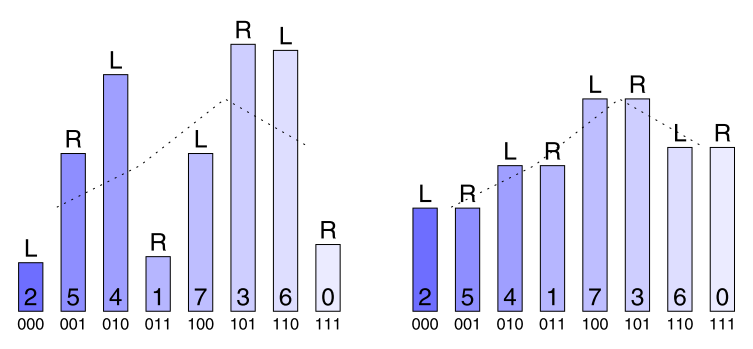
\includegraphics[width=90mm]{img/westfeld-histogram.png}
\caption{\label{fig:chi-histogram}Histograma das cores de uma imagem antes e depois de esteganografia com EzStego}
\legend{Fonte: \citeonline{westfeld1999attacks}}
\end{figure}

Um ponto crítico é como podemos obter a distribuição de frequências teoricamente esperada (i. e., a frequência de ocorrências que nós esperaríamos, após aplicarmos esteganografia)
 % A critical point is how to obtain the theoretically expected frequency distribution (i. e., the frequency of occurrence we would expect after applying stegano- graphic changes).
Essa frequência não pode ser derivada do item que está sendo análisado, porque ele pode ter sido alterado por operações esteganográficas.
 % This frequency must not be derived from our random sample, because this random sample could have been changed by steganographic op- erations.
Mas na maioria dos casos, nós não temos o arquivo original disponível para compararmos, ou para derivar a frequência esperada. No original, a frequência teoretica esperada é a média aritmética das duas frequências de um PoV.
 % But in most cases we don’t have the original to compare with or to derive the expected frequency from. In the original, the theoretically expected frequency is the arithmetic mean of the two frequencies in a PoV.
A linha tracejada na figura 14 conecta a média aritimética desses valores. Porque a esteganografia sobrescreve os LSBs, ela não muda a soma dessas duas frequências.
 % The dashed line in Fig. 14 connects these arithmetic mean values. Because the embedding function overwrites the least significant bits, it does not change the sum of these two frequencies.
O quantidade tirada dos valores ímpares é transferida para os valores pares correspondentes de cada PoV, e vice versa.
 % The count taken from the odd value frequency is transferred to the corresponding even value frequency in each PoV, and vice versa.
Como a soma é constante, a média aritmética também é a mesma para cada PoV. Tanto no arquivo original, quanto no arquivo alterado, o estanograma.
 % As the sum stays constant, the arithmetic mean is the same for a PoV in both, the original carrier medium and each corresponding steganogram.
Isso nos permite obter a distribuição de frequências teoricamente esperada através do item que está sendo analisado. Assim não precissamos do arquivo original para o ataque.
 % This fact allows us to obtain the theoretically expected frequency distribution from the random sample. So we don’t need the original carrier medium for the attack.


O gráu de similaridade entre a distribuição observada na amostra e a distribuição de frequências teoricamente esperada é a medida de probabilidade de que métodos estegaanográficos foram aplicados.
 % The degree of similarity of the observed sample distribution and the theoretically expected frequency distribution is a measure of the probability that some embedding has taken place.
Esse gráu de similaridade é determinado usando o teste Chi Square. Esse teste faz um mapeamento das observações em categorias.
 % The degree of similarity is determined using the Chi-square test (e.g., [1]). This test operates on a mapping of observations into categories. It performs the following steps:


\subsection{RS Analysis}
\cite{fridrich2001reliable}: detecta LSBs espalhados em imagens em tons de cinza ou coloridas ao inspecionar as diferenças no número de grupos regulares e singulares para os LSB e o plano LSB deslocado.

\subsection{Primary Sets}
\cite{dumitrescu2002steganalysis}: baseado em um identidade estatística relacionada a alguns conjuntos de pixels em uma imagem.

\subsection{Sample Pair}
\cite{dumitrescu2003detection}: baseado em uma máquina de estados finitos cujos estados são múltiplos conjuntos selecionados de pares de amostras chamados ``trace multisets''.


\section{Curva ROC}
%------------------




% % ----------------------------------------------------------
% % PARTE
% % ----------------------------------------------------------
% \part{Resultados}
% % ----------------------------------------------------------

% % ---
% % primeiro capitulo de Resultados
% % ---
% \chapter{Lectus lobortis condimentum}
% % ---

% % ---
% \section{Vestibulum ante ipsum primis in faucibus orci luctus et ultrices
% posuere cubilia Curae}
% % ---

% \lipsum[21-22]

% % ---
% % segundo capitulo de Resultados
% % ---
% \chapter{Nam sed tellus sit amet lectus urna ullamcorper tristique interdum
% elementum}
% % ---

% % ---
% \section{Pellentesque sit amet pede ac sem eleifend consectetuer}
% % ---

% \lipsum[24]

% ----------------------------------------------------------
% Finaliza a parte no bookmark do PDF
% para que se inicie o bookmark na raiz
% e adiciona espaço de parte no Sumário
% ----------------------------------------------------------
\phantompart

% ---
% Conclusão
% ---
\chapter{Conclusão}
% ---

\lipsum[31-33]

% ----------------------------------------------------------
% ELEMENTOS PÓS-TEXTUAIS
% ----------------------------------------------------------
\postextual
% ----------------------------------------------------------

% ----------------------------------------------------------
% Referências bibliográficas
% ----------------------------------------------------------
\bibliography{referencias}

% ----------------------------------------------------------
% Glossário
% ----------------------------------------------------------
%
% Consulte o manual da classe abntex2 para orientações sobre o glossário.
%
%\glossary

% ----------------------------------------------------------
% Apêndices
% ----------------------------------------------------------

% ---
% Inicia os apêndices
% ---
% \begin{apendicesenv}

% % Imprime uma página indicando o início dos apêndices
% \partapendices

% % ----------------------------------------------------------
% \chapter{Quisque libero justo}
% % ----------------------------------------------------------

% \lipsum[50]

% % ----------------------------------------------------------
% \chapter{Nullam elementum urna vel imperdiet sodales elit ipsum pharetra ligula
% ac pretium ante justo a nulla curabitur tristique arcu eu metus}
% % ----------------------------------------------------------
% \lipsum[55-57]

% \end{apendicesenv}
% ---


% ----------------------------------------------------------
% Anexos
% ----------------------------------------------------------

% ---
% Inicia os anexos
% ---
% \begin{anexosenv}

% % Imprime uma página indicando o início dos anexos
% \partanexos

% % ---
% \chapter{Morbi ultrices rutrum lorem.}
% % ---
% \lipsum[30]

% % ---
% \chapter{Cras non urna sed feugiat cum sociis natoque penatibus et magnis dis
% parturient montes nascetur ridiculus mus}
% % ---

% \lipsum[31]

% % ---
% \chapter{Fusce facilisis lacinia dui}
% % ---

% \lipsum[32]

% \end{anexosenv}

%---------------------------------------------------------------------
% INDICE REMISSIVO
%---------------------------------------------------------------------
\phantompart
\printindex
%---------------------------------------------------------------------

\end{document}
